
Un DataFrame est une structure de données étiquetée à deux dimensions avec des colonnes de types potentiellement différents. Un DataFrame peut-être une feuille de calcul, une table SQL ou un dictionnaire d'objets de série.

Ce TP vous invite à manipuler des dataframe à partir de fichiers externes.

\subsection{Fichiers de type texte (.txt)}




Pour manipuler un fichier texte, copiez/collez le fichier texte "biblo1.txt" dans le même fichier que le progromme et écrivez ce programme dans un éditeur de texte :

\lstinputlisting[language = python]{chapitre3/codes/texte.py}

La sortie écran obtenue est la suivante : 

\begin{figure}[H]
    \centering
    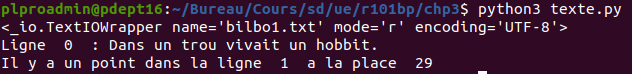
\includegraphics[scale = 0.5]{chapitre3/figures/texte.png}
\end{figure}

On retrouve les méthodes de manipulation des strings (chaînes de caractère), vues dans le chapitre précédent, et détaillées dans le manuel
\footnote{\url{https://www.w3schools.com/python/python_ref_string.asp}}.

\begin{tcolorbox}[lefttitle=2cm, colframe=gray!75!blue, title= \textbf{Tip for Code 1 : "\textit{les Droits}"}]

Les droits sur le fichier manipuler sont déclinés par les lettres suivantes :

r, pour une ouverture en lecture (READ).

w, pour une ouverture en écriture (WRITE), à chaque ouverture le contenu du fichier est écrasé. Si le fichier n'existe pas python le crée.

a, pour une ouverture en mode ajout à la fin du fichier (APPEND). Si le fichier n'existe pas python le crée.

b, pour une ouverture en mode binaire.

t, pour une ouverture en mode texte.

x, crée un nouveau fichier et l'ouvre pour écriture


\end{tcolorbox}


\begin{tcolorbox}[lefttitle=2cm, colframe=gray!50!red, title= \textbf{ WARNING}]
\textbf{Tout fichier ouvert (avec open) doit être fermé  (avec close).}

Tout oubli à ce sujet, vaudra une division par 2 de la note de l'exercice en question.
\end{tcolorbox}


\begin{tcolorbox}[lefttitle=2cm, colframe=gray!75!black, title= \textbf{Exercices}]
\textbf{1$\diamondsuit$-}
Le premier exercice vous invite à manipuler des fichiers textes.

\begin{enumerate}
    \item Mettre les fichiers textes "bilbo1.txt", "bilbo2.txt" et "bilbo3.txt" dans un dossier intitulé "fichiersTexte" dans le même dossier que votre programme. 
    \item Créer un nouveau fichier texte vide, appelé "bilbo.txt".
    \item Concaténer les 3 fichiers en un nouveau fichier "blibo.txt", lui-même placé dans le dossier "fichiersTexte".
\end{enumerate}

\textbf{2$\diamondsuit$-}
Modifier votre code de façon à créer le fichier texte "bilbo.txt" s'il n'est pas existant.

\textbf{3$\diamondsuit~\diamondsuit$-}
Modifier votre code afin de changer le mot "hobbit" par "Periannath" (langue elfique).

\textbf{(Optionnel)4$\diamondsuit~\diamondsuit$-}
Modifier votre programme afin d'intégrer, si ce n'est pas déjà fait, la librairie de gestion des fichiers "import os"\footnote{\url{https://docs.python.org/fr/3/library/os.html}} pour importer l'adresse du fichier courant. 

\textbf{(Optionnel)5$\diamondsuit~\diamondsuit~\diamondsuit$-}
Créer un programme qui prend en entrée un dossier. Et en sortie, ce programme affiche la hiérarchie des éléments au sein de ce dossier, avec le type de ces éléments (fichier, dossier, executable, ou autres).

\end{tcolorbox}

\subsection{Les fichiers csv}

Un fichier CSV (Comma-separated values) est un type de fichier associé à Excel. Plutôt que de stocker les informations en colonnes, les fichiers CSV les stockent en les séparant par des points-virgules.

Le csv utilié lors de ce TP est disponible sur le site de l'INSEE\footnote{\url{https://www.insee.fr/fr/statistiques/2540004?sommaire=4767262\#consulter}}
sous le lien : Fichier allégé par département depuis 2000. 


\begin{figure}[H]
    \centering
    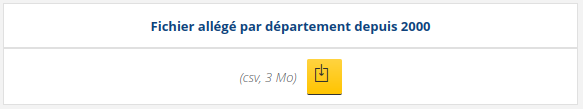
\includegraphics[scale = 0.5]{chapitre3/figures/csvINSEE.png}
\end{figure}

Télécharger l'archive dans un dossier intitulé "fichiersCSV", dans le même répertoire que celui contenant votre dossier "fichiersTexte".


Ensuite, copier le programme suivant :

\lstinputlisting[language = python]{chapitre3/codes/EcritureLecturecsv.py}

La sortie écran obtenue est la suivante : 

\begin{figure}[H]
    \centering
    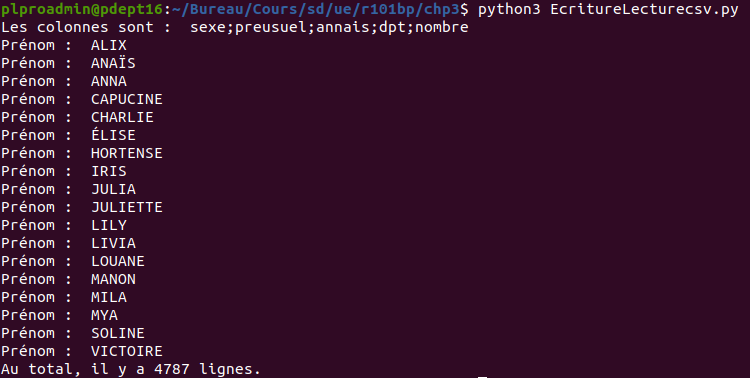
\includegraphics[scale = 0.5]{chapitre3/figures/csvex.png}
\end{figure}


\begin{tcolorbox}[lefttitle=2cm, colframe=gray!75!black, title= \textbf{Exercices}]
\textbf{1$\diamondsuit$-}
Le premier exercice vous invite à manipuler le programme précédent de façon à :

\begin{enumerate}
    \item Enumérer les prénoms féminins de 2021 qui apparaissent -cette fois- moins de 5 fois 
    \item Ecrire le résultat dans un fichier .txt, avec la mention "prénom rare" à côté, si le prénom apparaît moins de 4 fois.
\end{enumerate}

\textbf{(Optionnel) 2$\diamondsuit$-} Concaténer les deux cvs du Jura (39) et du Doubs (25) en un seul csv

\textbf{(Optionnel)3$\diamondsuit$-} Pourquoi vous ne devez pas appeler votre fichier python csv.py ?
\end{tcolorbox}

\subsection{Fichiers de type xlsx}

Le fichier xlsx est l'extension par défaut des fichiers créés avec la version 2007 du logiciel Excel.

Le xlsx utilié lors de ce TP est disponible sur le site de l'INSEE\footnote{\url{https://www.insee.fr/fr/statistiques/6011070?sommaire=6011075}}
sous le lien : France hors Mayotte. 


\begin{figure}[H]
    \centering
    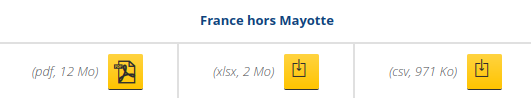
\includegraphics[scale = 0.5]{chapitre3/figures/xlsxTl.png}
\end{figure}

Télécharger le fichier dans un dossier intitulé "fichiersXLSX", dans le même répertoire que celui contenant vos dossiers "fichiersTexte" et "fichiersCSV".

Ensuite, copier le programme suivant :

\lstinputlisting[language = python]{chapitre3/codes/EcritureLecturexlsx.py}


\begin{tcolorbox}[lefttitle=2cm, colframe=gray!75!black, title= \textbf{Exercice}]
Pourquoi il est déconseillé d'écrire L 22 : " if x.startswith('Dol') and type(x) == str:"  ?
\vspace{2cm}
\end{tcolorbox}



La sortie écran obtenue est la suivante : 

\begin{figure}[H]
    \centering
    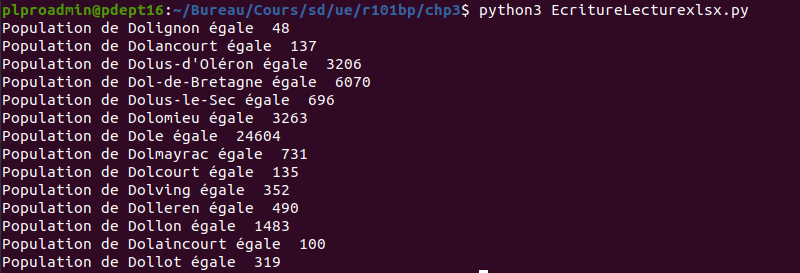
\includegraphics[scale = 0.5]{chapitre3/figures/xlsxCE.png}
\end{figure}

On retrouve les méthodes de manipulation des strings (chaînes de caractère), vues dans le chapitre précédent, et détaillées dans le manuel
\footnote{\url{https://www.w3schools.com/python/python_ref_string.asp}}.

De plus, on utilise la méthode enumerate \footnote{\url{https://docs.python.org/3/library/functions.html\#enumerate}} pour accéder aux index de la boucle (voir chapitre précédent). 

\begin{tcolorbox}[lefttitle=2cm, colframe=gray!75!blue, title= \textbf{Tip for Code 2 : "\textit{Panel Data}"}]


La bibliothèque logicielle open-source Pandas est spécifiquement conçue pour la manipulation et l’analyse de données en langage Python. Elle est à la fois performante, flexible et simple d’utilisation.

Grâce à Pandas, le langage Python permet enfin de charger, d’aligner, de manipuler ou encore de fusionner des données. Les performances sont particulièrement efficaces quand le code source back-end est écrit en C ou en Python.

Le manuel est disponible à cette adresse :
\url{https://pandas.pydata.org/docs/reference/api/pandas.ExcelFile.html}

\end{tcolorbox}




\begin{tcolorbox}[lefttitle=2cm, colframe=gray!75!black, title= \textbf{Exercices}]
\textbf{1$\diamondsuit$-}
Le premier exercice vous invite à manipuler le programme précédent de façon à :
Afficher sur le terminal la population totale des villes commençant par "Dol"

    
\textbf{(Optionnel)2$\diamondsuit~\diamondsuit$-} 
On s'intéresse en suite aux communes dont la commune pôle est Mièges (Mièges comprise), dans la feuille "Communes associées ou déléguées".
Créer un fichier texte contenant :
\begin{enumerate}
    \item le nombre de ces communes
    \item leur nom, leur population municipale et leur population totale
    \item si leur population comptée à part est null, rajouter la mention "urbain"
    \item afficher la population totale
\end{enumerate}

    
\textbf{(Optionnel)3$\diamondsuit~\diamondsuit~\diamondsuit$-} 
Creer un nouveau fichier xlsx, de façon à avoir les colonnes de la feuille "Communes associées ou déléguées", avec le numéro de Canton (dans la feuille "Communes").

Vous rajouterez également une visualisation de la population de votre choix en utilisant la bibliothèque plot \footnote{\url{https://pandas.pydata.org/docs/user_guide/visualization.html}}.


\textbf{(Optionnel)4$\diamondsuit$-} Pourquoi vous ne devez pas appeler votre fichier python csv.py ?
\end{tcolorbox}


\subsection{Fichiers de type json }




\begin{tcolorbox}[lefttitle=2cm, colframe=gray!50!yellow, title= \textbf{ JSON}]
Le JavaScript Object Notation (JSON) est un format standard utilisé pour représenter des données structurées de façon semblable aux objets Javascript.
Un json est représenté par une liste de dictionnaires.

\begin{figure}[H]
    \centering
    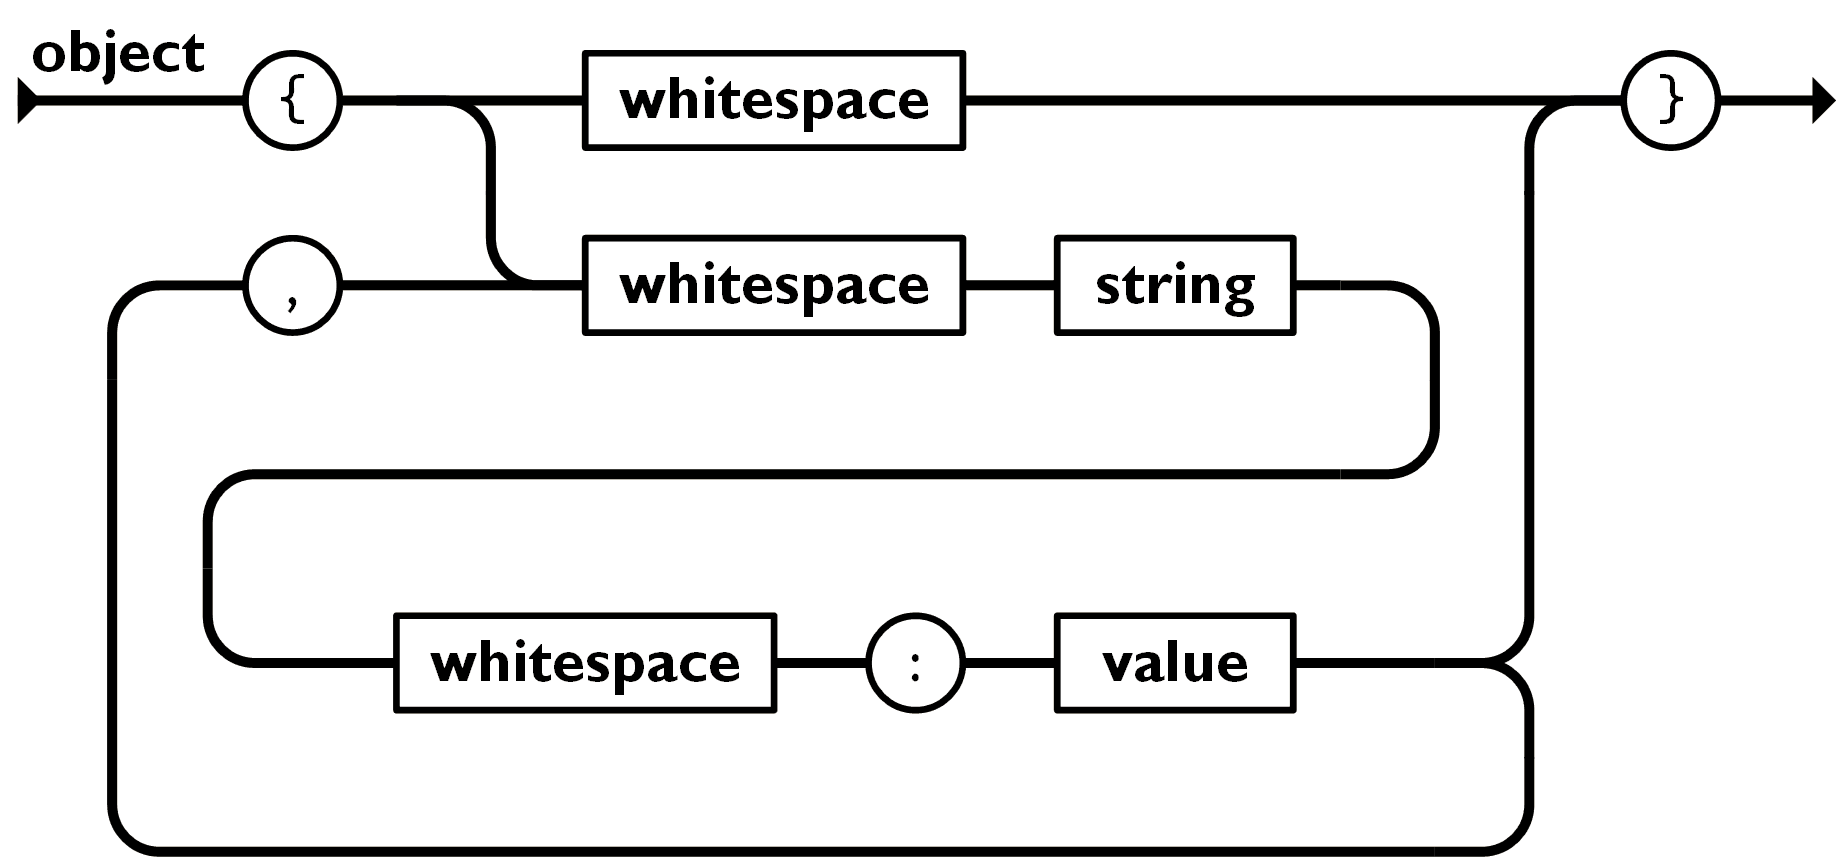
\includegraphics[scale = 0.5]{chapitre3/figures/jsonImg.png}
\end{figure}

\end{tcolorbox}


Pour cet exercice, copier le programme suivant : 
\lstinputlisting[language = python]{chapitre3/codes/EcritureLecturejson.py}

La sortie écran obtenue est la suivante : 

\begin{figure}[H]
    \centering
    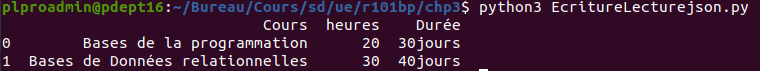
\includegraphics[scale = 0.5]{chapitre3/figures/json.png}
\end{figure}

\begin{tcolorbox}[lefttitle=2cm, colframe=gray!75!black, title= \textbf{Exercice}]
\textbf{1$\diamondsuit$-}
A partir du manuel\footnote{\url{https://pythonbasics.org/pandas-json/}} et du programme précédent, rajouter le numéro de semestre correspondant au cours et les notes de ces matières.

\end{tcolorbox}


\newpage

\subsection{Bilan (obligatoire)}



\makebox[0.75\textwidth]{Lors de ce TP, vous vous êtes arrêté à quel exercice ? \enspace\hrulefill}


\makebox[1\textwidth]{--------------------------------------------------Remplir le tableau--------------------------------------------------}

\textbf{Partie savoir faire}
\begin{itemize}
    \item Niveau 1 : Je n'ai pas su l'implémenter. C'est du charabiah pour moi. 
    \item Niveau 2 : J'ai lu le sujet. Les couleurs sont jolies. J'ai fini le premier exercice les yeux rivés sur mon clavier pour chercher les touches. Les erreurs de l'interpréteur me semblent incompréhensibles.
    \item Niveau 3 : J'ai pu avancer à la moitié du sujet, même si c'est difficile et que l'ordi est farceur (comme tous les ordis). Je prends beaucoup de temps à comprendre les erreurs du shell, mais j'y arrive !
    \item Niveau 4 : J'ai complété le TP avec aisance. La plupart des erreurs du shell me sont compréhensibles.
    \item Niveau 5 : J'ai complété le TP, exercices optionnels compris ! J'ai une grande agilité\footnote{agilité $\rightarrow$ ne pas utiliser la souris en codant} quand je code. 
\end{itemize}


\textbf{Partie savoir être}
\begin{itemize}
    \item Niveau 1 :  Pour finir au plus vite, j'élabore des stratégies (copier directement la réponse ou chercher à camoufler le désintérêt : "Si je n'y arrive pas, c'est que le prof n'est pas venu assez vite me donner la solution"). 
    \item Niveau 2 : L'objectif est d'avoir la moyenne sans trop y laisser du temps ou de l'énergie. Je suis bien obligé de faire le TP, même si l'idée de me servir du pannel de ressources me semble saugrenue. Si c'est possible de récupérer la réponse (ou de suivre à côté d'un camarade\footnote{Mais si, c'est du travail d'équipe : il code et je le soutiens émotionnellement !}), alors je ne dirai pas non. 
    \item Niveau 3 : Je prends doucement mes marques. Je me suis servi de façon hésitante de plusieurs ressoures dispos (shell, camarades, enseignants, manuel, sites web, ou même canard\footnote{\url{https://fr.wikipedia.org/wiki/M\%C3\%A9thode_du_canard_en_plastique}}) en cherchant à comprendre leur réponse. J'aimerais un jour pouvoir développer  mes propres projets et il faut pour cela que je gagne en autonomie.
    \item Niveau 4 :   Je suis autonome dans l'utilisation des ressoures disponibles (shell, camarades, enseignants, manuel, sites web, ou même canard\footnotemark[7]). J'ai même un projet personnel en cours que j'aimerais finir.
    \item Niveau 5 : J'évolue avec aisance dans cet environnement ! Je  fais même partie dorénavant des ressoures dispos et  j'échange facilement sur ces notions. J'ai plusieurs projets informatiques personnels. 
\end{itemize}

\begin{table}[H]
    \centering
    \begin{tabular}{|c|c|c|} \hline
        \textbf{Notions} & \textbf{Niveau atteint} (de 1 à 5) \textbf{Savoir faire}  & \textbf{Niveau atteint} (de 1 à 5) \textbf{Savoir être}\\\hline
        txt & & \\\hline
        csv &&\\\hline
        xlsx &&\\\hline
        json &&\\\hline
        Respect des règles de bon codage && \\\hline
    \end{tabular}
\end{table}


